%{{{ Formatierung

\documentclass[a4paper,10pt]{article}

\usepackage{physics_notetaking}

%%% dark red
%\definecolor{bg}{RGB}{60,47,47}
%\definecolor{fg}{RGB}{255,244,230}
%%% space grey
%\definecolor{bg}{RGB}{46,52,64}
%\definecolor{fg}{RGB}{216,222,233}
%%% purple
%\definecolor{bg}{RGB}{69,0,128}
%\definecolor{fg}{RGB}{237,237,222}
%\pagecolor{bg}
%\color{fg}

\newcommand{\td}{\,\text{d}}
\newcommand{\RN}[1]{\uppercase\expandafter{\romannumeral#1}}
\newcommand{\zz}{\mathrm{Z\kern-.3em\raise-0.5ex\hbox{Z} }}
\newcommand{\id}{1\kern-.258em1}

\newcommand\inlineeqno{\stepcounter{equation}\ {(\theequation)}}
\newcommand\inlineeqnoa{(\theequation.\text{a})}
\newcommand\inlineeqnob{(\theequation.\text{b})}
\newcommand\inlineeqnoc{(\theequation.\text{c})}

\newcommand\inlineeqnowo{\stepcounter{equation}\ {(\theequation)}}
\newcommand\inlineeqnowoa{\theequation.\text{a}}
\newcommand\inlineeqnowob{\theequation.\text{b}}
\newcommand\inlineeqnowoc{\theequation.\text{c}}

\renewcommand{\refname}{Source}
\renewcommand{\sfdefault}{phv}
%\renewcommand*\contentsname{Contents}

\pagestyle{fancy}

\sloppy

\numberwithin{equation}{section}

%}}}

\begin{document}

%{{{ Titelseite

\begin{titlepage}
        \title{1 $|$ Ausbreitung von Signalen auf Leitungen}
        \author[1]{Angelo Brade\thanks{s72abrad@uni-bonn.de}}
        \author[1]{Jonas Wortmann\thanks{s02jwort@uni-bonn.de}}
        \affil[1]{Rheinische Friedrich--Wilhelms--Universität Bonn}
        \date{\today}
\end{titlepage}

\maketitle
\pagenumbering{gobble}

%}}}

\newpage

%{{{ Inhaltsverzeichnis

\fancyhead[R]{\thepage}
\fancyfoot[C]{}

\tableofcontents

%}}}

\newpage

%{{{

\pagenumbering{arabic}
\fancyhead[L]{\leftmark}

\section{Einleitung}
In diesem Versuch werden Koaxialkabel und ihre Eigenschaften behandelt.
Die Reflexionseigenschaften innerhalb von Koaxialkablen sollen verstanden, sowie die spezifische Dämpfung von Klippkabeln gemessen werden.
Zudem wird das Rechtecksignal eines Hochpasses differenziert und das Verhalten bei verschiedenen vorgeschalteten Widerständen beobachtet.

\newpage
\section{Theorie}
Eine Doppelleitung (Hin-- und Rückleiter), deren elektrische Eigenschaften längs der ganzen Strecke gleichbleiben, nennt man homogene Leitung.
Koaxialkabel sind homogene Leitungen und bestehen aus einem leitenden Draht in der Mitte, darum ein Dielektrikum und wieder darum ein Geflecht aus einem leitenden Material welches Strahlung abschirmt.
Das ganze Kabel ist isoliert.
\\\indent Kabel können auch näherungsweise über eine Kette von LC--Gliedern dargestellt werden.
Hier verteilt sich die gesamte Induktivität und Kapazität über das gesamte Kabel.
Ein Ersatzschaltbild für die Wellenausbreitung in einem Leiter ist
\begin{figure}[h]
        \centering
        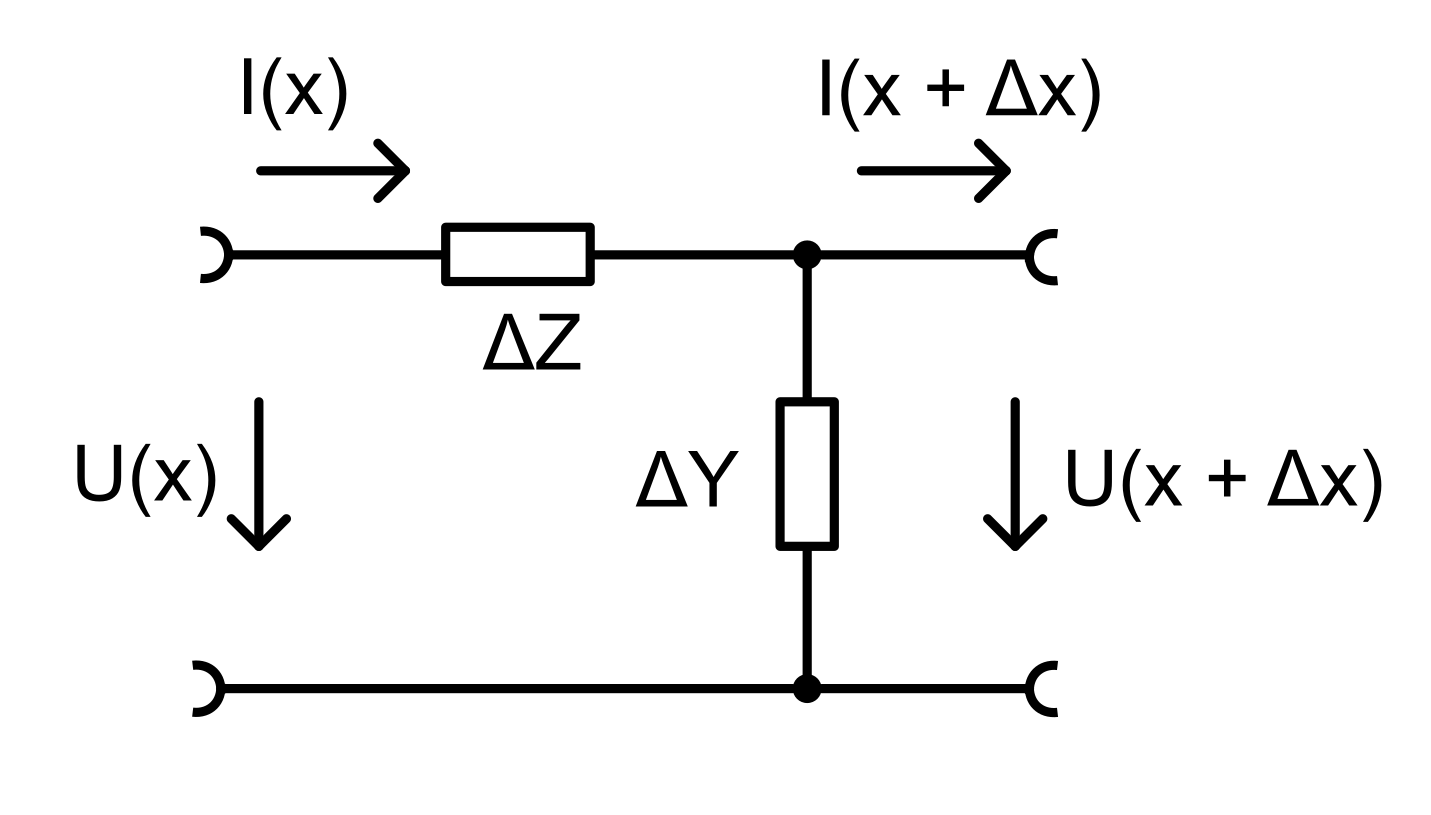
\includegraphics[width=0.6\textwidth]{ersatz_wellenausbreitung.png}
        \caption{Ersatzschaltbild zur Wellenausbreitung; Abbildung 1.3 \cite{Praktikumsanleitung}}
\end{figure}\\
Der Wellenwiderstand eines Kabels ist definiert als 
\begin{align} 
        Z=\dfrac{U_h\left(x\right)}{I_h\left(x\right)}=\dfrac{U_r\left(x\right)}{-I_r\left(x\right)}
,\end{align} 
mit $_h$ der Hinrichtung und $_r$ der Rückrichtung.
Im verlustfreien Fall ist $Z=\,\sqrt[]{\tfrac{L'}{C'}}$, also rein reell.
Für ein Koaxialkabel mit Innenradius $R_i$ und Außenradius $R_a$ gilt
\begin{align} 
        Z=Z_\text{frei}\cdot \dfrac{\ln\left(\tfrac{R_a}{R_i}\right)}{2\pi }
,\end{align} 
wobei $Z_\text{frei}=\,\sqrt[]{\tfrac{\mu _0}{\varepsilon _0}}=120\pi \,\SI{}{\ohm}$ der Wellenwiderstand des Vakuums ist.
\\\indent Es existieren drei verschiedene wichtige Möglichkeiten für den Abschlusswiderstand in einer Leitung.
\begin{enumerate}[label=--]
        \item Angepasster Abschluss: $R_A=Z,r=0,s=1,m=1$. 
                Hier sieht es für die einhegende Welle so aus, als würde der Widerstand $R_A$ das Kabel fortführen.
                Es kommt zu keiner Reflexion der Welle (siehe $r=0$).
        \item Offene Leitung: $R_A=\infty,r=+1,s=\infty,m=0$.
                Bei einer offenen Leitung ist kein Widerstand an das Ende des Kabels angeschlossen.
                Hier wird die Welle mit gleicher Polarisation reflektiert und interferiert dann mit der eingehenden Welle konstruktiv.
        \item Kurzschluss: $R_A=0,r=-1,s=\infty,m=0$.
                Bei einem Kurzschluss wird die Welle mit umgekehrter Polarisation reflektiert und interferiert desstruktiv mit der eingehenden Welle.
\end{enumerate}
Hier beschreiben $R_A$ den Abschlusswiderstand, $r$ den Reflexionskoeffizienten, $s$ das Stehwellenverhältnis und $m$ den Anpassungsfaktor.\\\\
In Klippkabeln kann die Länge eines Impulses sowie die Dämpfung variiert werden.
Die Dämpfung ist bestimmt über das Verhältnis der Eingangsspannung zur Ausgangsspannung
\begin{align} 
        20\,\log\left(\dfrac{U_\text{out}}{U_\text{in}}\right)
.\end{align} 
Einige Beispiele für spezifische Dämpfungen finden sich in (\ref{fig:literatur}). 

\newpage
\section{Voraufgaben}
\subsection{A}
Um große Verzögerungszeiten zu erreichen muss eine kleine Phasengeschwindigkeit sichergestellt werden, entsprechend große Permeabilität und Permitivität.

\subsection{B}
Wird die Verzögerungszeit über die Phasengeschwindigkeit geändert, so ändert sich auch der Wellenwiderstand, da diese Größen verschiedene Proportionalitäten besitzen
\begin{align} 
        v_{\text{ph}}\propto \dfrac{1}{\,\sqrt[]{L'C'}}\qquad Z\propto \,\sqrt[]{\dfrac{L'}{C'}}
.\end{align} 
Das Aufwickeln des Innenleiters um einen Ferritkern damit die Induktivität des Kabels gesteigert wird ändert den Wellenwiderstand nicht.

\subsection{C}
Sei ein Kabel abgeschlossen mit $R_A=Z$, findet keine Reflexion statt.
Alle Energie, die am Eingang des Kabels einläuft, wird am Kabelende vollständig an den Verbraucher $R_A$ abgegeben, da dieser wie eine Fortsetzung des Kabels aussieht.
Der Eingangswiderstand ist hier also unabhängig von der Länge des Kabels.

\subsection{D}
Sei ein verlustfreier idealer Leiter mit den Eigenschaften $\tfrac{R_A}{R_I}=2.3,\varepsilon _r=1.5$ und $\mu _r=1.5$.
Dann ist die Phasengeschwindigkeit
\begin{align} 
        v_{\text{ph}}&=\dfrac{c_0}{\,\sqrt[]{\varepsilon _r\mu _r}}=\dfrac{c_0}{1.5}\approx \SI{1.93e+8}{m.s ^{-1}}
,\end{align} 
der Wellenwiderstand
\begin{align} 
        Z=\,\sqrt[]{\dfrac{L'}{C'}}=\,\sqrt[]{\dfrac{\mu _r\mu _0}{\varepsilon _r\varepsilon _0}\dfrac{\ln^2\left(R_a/R_i\right)}{4\pi ^2}}\approx \SI{49.94}{\ohm}
\end{align} 
und die Verzögerung
\begin{align} 
        \Delta =\dfrac{1}{v_{\text{ph} }}=\dfrac{1.5}{c_0}\approx \SI{5.2e-9}{s.m ^{-1}}\approx \SI{5.2}{\nano s.m ^{-1}}
.\end{align} 


\newpage
\section{Auswertung}

\subsection{Versuchsaufgabe 1: Differenzierglied}
Wir erzeugen Impulse, indem wir ein Rechtecksignal mithilfe eines Differenzierglieds ableiten. Es sind 200 kHz bei 10 V eingestellt. Ein Ausschnitt ist in Abb. \ref{fig:1.1} gezeigt.
\begin{figure}[h]
        \centering
        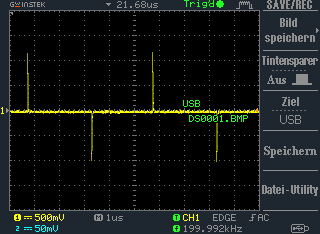
\includegraphics[width=0.6\textwidth]{data/DS0001.BMP.png}
        \caption{Impulse als Ableitung des Rechtecksignals}
		\label{fig:1.1}
\end{figure}\\
Wenn wir nun den eingebauten 2.2 k$\Omega$ Widerstand verwenden, sehen wir eine deutliche Verkleinerung des Rignals (betrachte die gelbe Skalar: 50 mV im Vergleich zu 500 mV von zuvor). Dieses ist wieder in Abb. \ref{fig:1.2} dargestellt. Zusätzlich können wir eine Abklinkzeit beobachten. Dies ist auch plausibel, da Widerstände Dämpfen, sowie die Konstruktion nicht mehr annähand Verlustfrei machen und so eine sichbare Verzögerung/Abklinkzeit hinzukommt.
\begin{figure}[h]
        \centering
        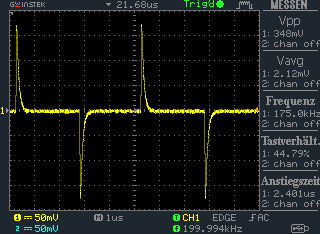
\includegraphics[width=0.6\textwidth]{data/DS0003.BMP.png}
        \caption{Impulse mit Widerstand}
		\label{fig:1.2}
\end{figure}

\subsection{Versuchsaufgabe 2: Impulse auf Kabeln}
Es wird eine Schaltung nach Abb. \ref{fig:2.1} aufgebaut, um Impulse an beiden Enden hin- und herlaufen zu lassen.
\begin{figure}[h]
        \centering
        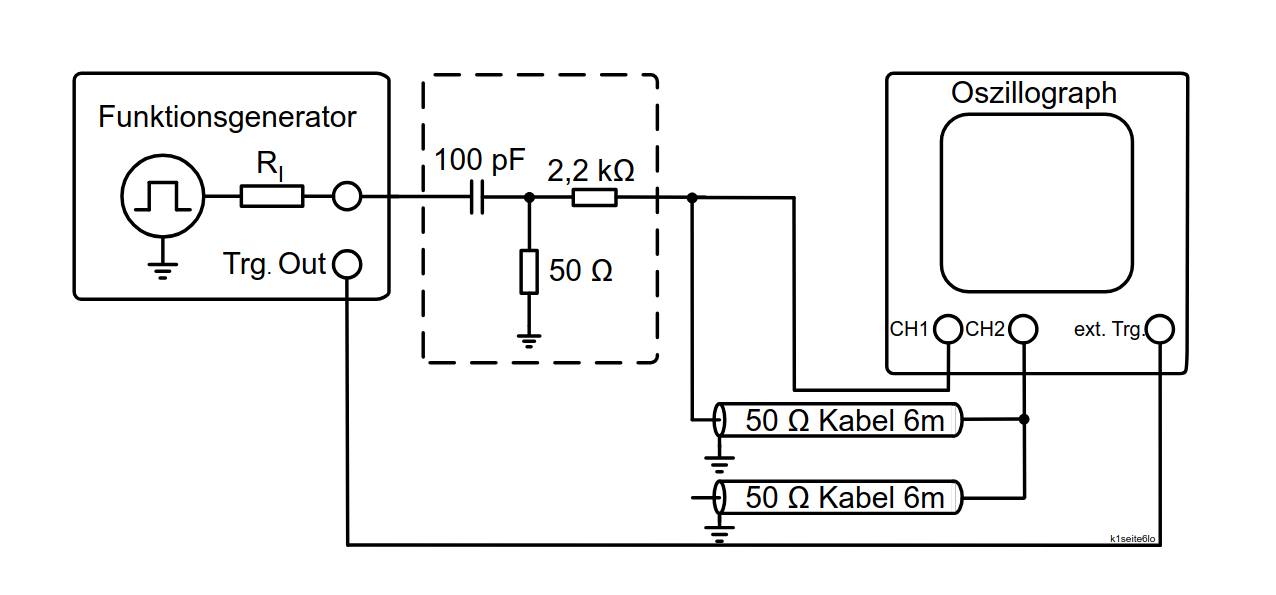
\includegraphics[width=0.6\textwidth]{Schaltung_offen.png}
        \caption{Schaltung mit offenen Enden}
		\label{fig:2.1}
\end{figure}
An dem Signalgenerator stellen wir 100 kHz und 20V ein.
\begin{figure}[h]
        \centering
        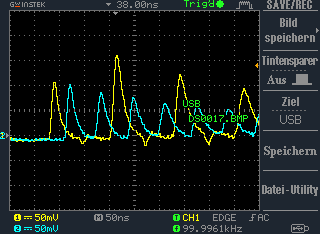
\includegraphics[width=0.6\textwidth]{data/DS0017.BMP.png}
        \caption{Schaltung mit offenen Enden}
		\label{fig:2.2}
\end{figure}\\
Bei dem Urspungssignal sehen wir, dass es mit einem größerem Peak und dann mit kleineren Peaks nachhallt. Das zweite Signal, welches durch die Kabel gedämpft wird, hier in blau in Abb. \ref{fig:2.2}, zieht um einen Versatz dem Ursprungssignal nach und beinhaltet zusätzlich die rückläufige Welle. So lassen sich pro Ursprungssignal, zwei weitere Peaks dem blauen Signal entnehmen. Die rückläufige Welle entsteht aufgrund des offenen Leiter-Endes, welches als Glanzfläche, die einlaufende Welle phasengleich reflektiert. Einen Abstieg der Amplituden lässt sich aufgrund der Dämpfung - des Widerstands im Kabel - erklären.

\subsection{Versuchsaufabe 3: Leitungsabschluss, Verzögerungszeit}
Zur Untersuchng verschiedener Leitungsabschlüsse wird die Schaltung nach Abb. \ref{fig:3.1} konstruiert. 
\begin{figure}[h]
        \centering
        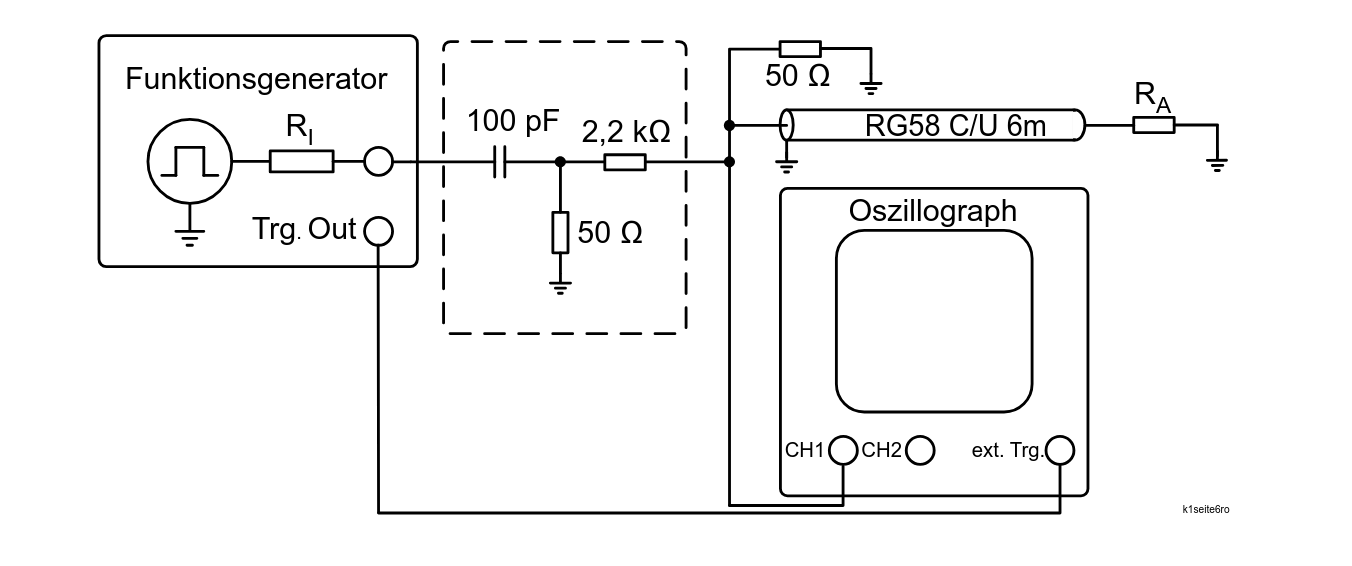
\includegraphics[width=0.6\textwidth]{Schaltung_Abschluss.png}
        \caption{Schaltung mit offenen Enden}
		\label{fig:3.1}
\end{figure}\\
\indent Vorerst ist hierbei das Verzögerungskabel offen. Wir erhlaten die in Abb. \ref{fig:3.2} gezeigte Spannung.
\begin{figure}[h]
        \centering
        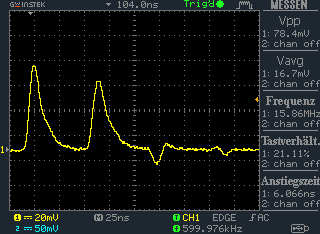
\includegraphics[width=0.6\textwidth]{data/DS0018.BMP.png}
        \caption{Einzelner Impuls mit Nachschwingung}
		\label{fig:3.2}
\end{figure}
\begin{figure}[h]
        \centering
        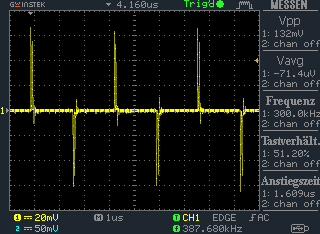
\includegraphics[width=0.6\textwidth]{data/DS0021.BMP.png}
        \caption{Mehrere Impulse mit Nachschwingung}
		\label{fig:3.3}
\end{figure}\\
Hierbei ist klar der eigentliche Impuls, sowie die Nachschwingung (zweiter Peak) zu erkennen.
\indent Schließen wir nun das Kabel mit einem 50 $\Omega$ ab, so können wir in Abb. \ref{fig:3.4} erkennen, dass es keine Nachschwingung gibt und das Kabel aus der eigenen Sicht unendlich weitergeführt wird. 
\begin{figure}[h]
        \centering
        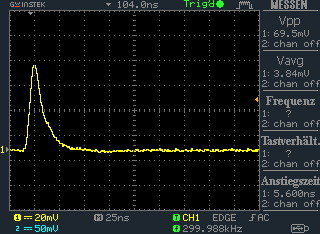
\includegraphics[width=0.6\textwidth]{data/DS0019.BMP.png}
        \caption{Einzelner Impuls ohne Nachschwingung}
		\label{fig:3.4}
\end{figure}
\begin{figure}[h]
        \centering
        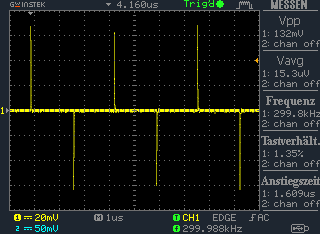
\includegraphics[width=0.6\textwidth]{data/DS0020.BMP.png}
        \caption{Mehrere Impulse ohne Nachschwingung}
		\label{fig:3.5}
\end{figure}\\
\indent Lassen wir nun das Kabel in einem Kurzschluss enden, so kann man in Abb. \ref{fig:3.6} die rücklaufende gegenphasige Nachschwingung erkennen.
\begin{figure}[h]
        \centering
        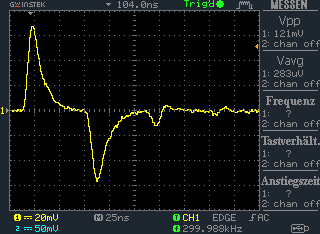
\includegraphics[width=0.6\textwidth]{data/DS0023.BMP.png}
        \caption{Einzelner Impuls mit gegenphasiger Nachschwingung}
		\label{fig:3.6}
\end{figure}
\begin{figure}[h]
        \centering
        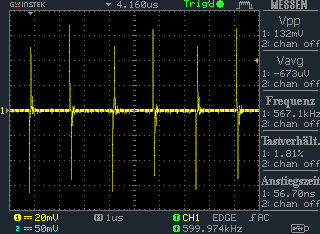
\includegraphics[width=0.6\textwidth]{data/DS0022.BMP.png}
        \caption{Mehrere Impulse mit gegenphasiger Nachschwingung}
		\label{fig:3.7}
\end{figure}\\
Diese gegenphasige Nachschiwngung ist aufgrund des kleineren Widerstandes zu erklären, da bei einem Kurzschluss der Widerstand praktisch Null und somit kleiner dem Wellenwiderstand ist. 

Variieren wir nun die Frequenz, so erhalten wir mit einer kleineren Frequenz (2 MHz) Abb. \ref{fig:3.8} und mit einer höheren Frequzenz (2.7MHz) Abb. \ref{fig:3.9}
\begin{figure}[h]
        \centering
        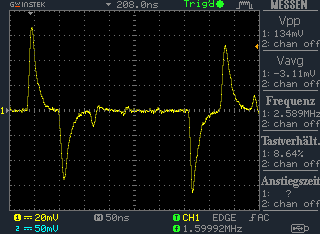
\includegraphics[width=0.6\textwidth]{data/DS0024.BMP.png}
        \caption{Einzelner Impuls mit gegenphasiger Nachschwingung}
		\label{fig:3.8}
\end{figure}
\begin{figure}[h]
        \centering
        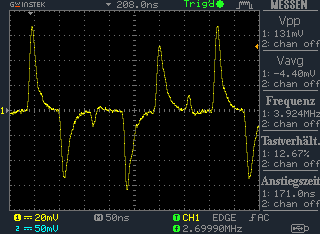
\includegraphics[width=0.6\textwidth]{data/DS0025.BMP.png}
        \caption{Mehrere Impulse mit gegenphasiger Nachschwingung}
		\label{fig:3.9}
\end{figure}

Es ist deutlich zu erkennen, dass der Abstand der Impulse sich verkleinert und die Abstände zwischen einem Einzelnen Impuls und der korrespondierenden Nachschwingung gleich bleibt. Dies ist zu erwarten, da die Erhöhung der Frequenz einfach mehr Impulse produziert. Andereseits ändert sich der Abstand zwischen den Nachschwingungen und dem Ursprungssignal nicht, da die Nachschwingung, in Relation zu dem Ursprungssignal, unabhängig von der Freqzenz ist. Anders gesagt, die Nachschwingung wird von der Frequenzänderung im gleichen Maße verschoben, wie der Impuls selber, sie bleiben also in Relation zu einander gleich.

Den Abbildungen kann man eine Zeitdifferenz von 64(4) ns, zwischen Impuls und Nachschwingung, entnehmen. Da das Signal das 6m lange Kabel zweimal durchlaufen muss, erhalten wir als Verzögerungszeit 5.3(3) ns. Dies deckt sich mit dem Literaturwert von 5.0(1) ns gut.

Mit einem Abschluss durch einen Wellenwiderstand würden wir nun keine Nachschwingung erwarten, da die Energie der Schwingung vollständig im Widerstand absorbiert wird. Dies Vermutung wurde getestet und in Abb. \ref{fig:3.10} gezeigt.
\begin{figure}[h]
        \centering
        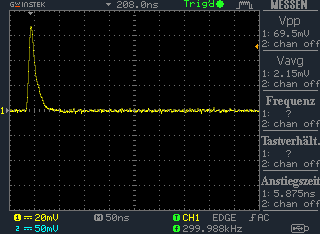
\includegraphics[width=0.6\textwidth]{data/DS0026.BMP.png}
        \caption{Einzelner Impulse mit abgeschlossenem Kabel}
		\label{fig:3.10}
\end{figure}\\
Unsere Vermutung lässt sich mit der Abb. bestätigen.

\clearpage
\subsection{Versuchsaufgabe 4: Klippkabel, Dämpfung}
In diesem Veruchsteil werden Klippkabel verwendet, die es möglich machen die Länge von Impulsen zu variieren.
\begin{figure}[h]
        \centering
        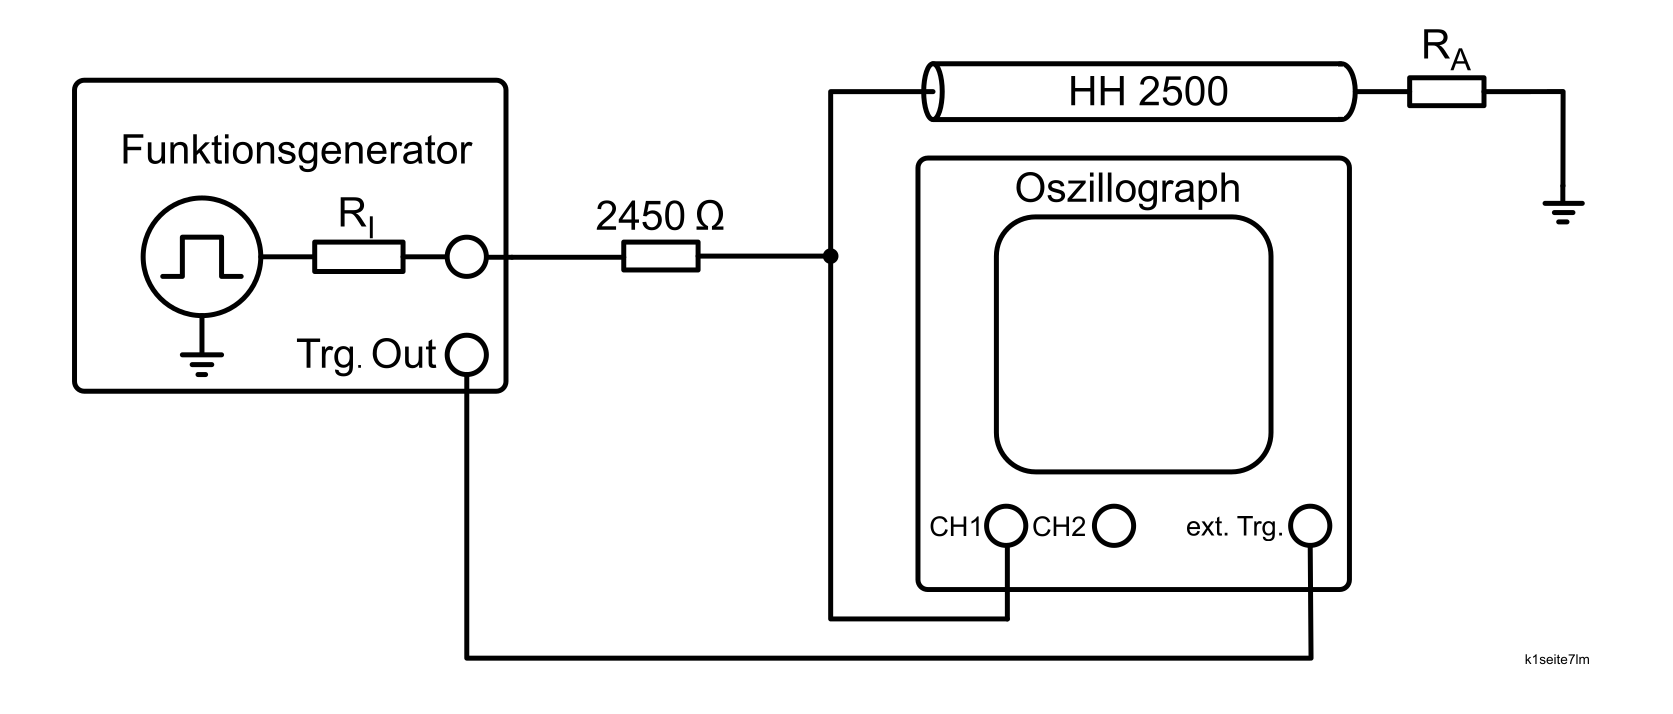
\includegraphics[width=\textwidth]{versuchsaufgabe4.png}
        \caption{Aufbau mit Klippkabel}
\end{figure}\\
Die Frequenz des Funktionsgenerators liegt bei $\SI{40}{kHz}$.\\\\
Zunächst bleibt das $\SI{2500}{\ohm}$ Klippkabel offen.
Das Rechtecksignal hat die folgende Form
\begin{figure}[h]
        \centering
        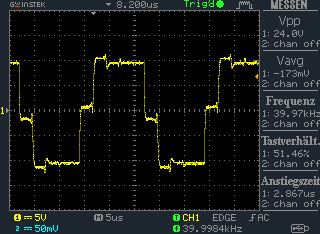
\includegraphics[width=0.6\textwidth]{data/DS0028.BMP.png}
        \caption{Rechtecksignal durch offenes Klippkabel}
\end{figure}\\
Das Signal, welches auf dem Oszillographen angezeigt wird ist eine Überlagerung der hin-- und rücklaufenden Welle durch das Klippkabel.
Es lässt sich erkennen, dass im drei Plateaus vorhanden sind.
Die größten Amplituden (in positive als auch negative Richtung) sind die Amplituden des Rechtecksignals gleicher Polarisation beider Wellen.
Die Amplituden um die Nulllage herum, entstehen durch destruktive Interferenz beider Signale, da eine Phasendifferenz zwischen dem hin-- und rücklaufenden Signal vorhanden ist.\\\\
Schließt man das Verzögerungskabel kurz entsteht folgendes Bild
\begin{figure}[h]
        \centering
        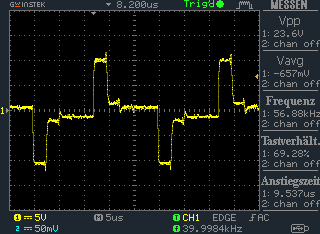
\includegraphics[width=0.6\textwidth]{data/DS0031.BMP.png}
        \caption{Signal mit kurzgeschlossenem Klippkabel}
\end{figure}\\
Bei einem Kurzgeschlossenen Ende des Kabels wird die Welle um $\SI{180}{\degree}$ Phasenverschoben reflektiert (Reflexionskoeffizient $r=-1$).
Das bedeutet, dass der Großteil des Signals durch destruktive Interferenz verschwindet und nur kleine Peaks bleiben, bei denen sich die Wellen aufgrund von Verzögerung noch konstruktiv Überlagern.\\\\
Variiert man die Frequenz des Funktionsgenerators, so bleibt die Größe der Impulse selbst gleich, nur die Abstände zwischen den Impulsen verändert sich.
Das kommt daher, dass sich die Frequenz des Funktionsgenerators nur auf die Anzahl der Impulse und nicht ihre Länge bezieht.\\\\
Nun werden drei $\SI{70}{cm}$ Klippkabel in Reihe geschalten, um ein $\SI{2}{m}$ langes Klippkable zu erzeugen.
Die Länge der Impulse ist in diesem Fall nur von der Länge der Klippkabel bestimmt.
Die Zeit zwischen zwei Impulsen erhöht sich bei einem längeren Klippkabel.\\\\
Die Dämpfung des Klippkabels bemerkt man an den Höhenunterschieden der Plateaus um die Nulllage herum (\ref{fig:dämpfung_anschaulich}).
Um die spezifische Dämpfung des Kabels zu berechnen kann die Spitze--Spitze Spannung mit der Eingangsspannung verglichen werden.
In (\ref{fig:dämpfung}) erkennt man eine Spitze--Spitze Spannung von $U_\text{out}=\SI{18}{V}$.
Es gilt bei einer Eingangsspannung von $U_\text{in}=\SI{20}{V}$ mit einer Frequenz von $\SI{200}{\kilo Hz}$
\begin{align} 
        D=20\log\left(\dfrac{U_\text{out}}{U_\text{in}}\right)\dfrac{1}{l}=20\log\left(\dfrac{\SI{18}{V}}{\SI{20}{V}}\right)\dfrac{1}{\SI{2}{m}}\approx 0.458
.\end{align} 
Vergleicht man mit den Literaturwerten (\ref{fig:literatur}), erkennt man, dass der berechnete Wert für die Dämpfung pro Meter des Kabels genau auf der Linie für das HH2500 Kabel liegt.
\begin{figure}[h]
        \centering
        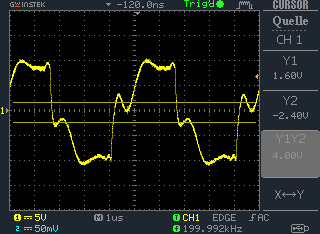
\includegraphics[width=0.6\textwidth]{data/DS0038.BMP.png}
        \caption{Dämpfung eines Klippkabels, veranschaulicht}\label{fig:dämpfung_anschaulich}
\end{figure}
\begin{figure}
        \centering
        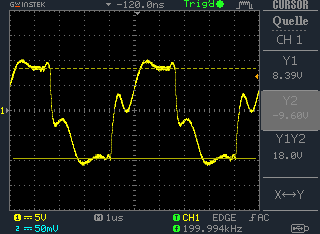
\includegraphics[width=0.6\textwidth]{data/DS0039.BMP.png}
        \caption{Dämpfung anhand der Spitze--Spitze Spannung}\label{fig:dämpfung}
\end{figure}
\begin{figure}[h]
        \centering
        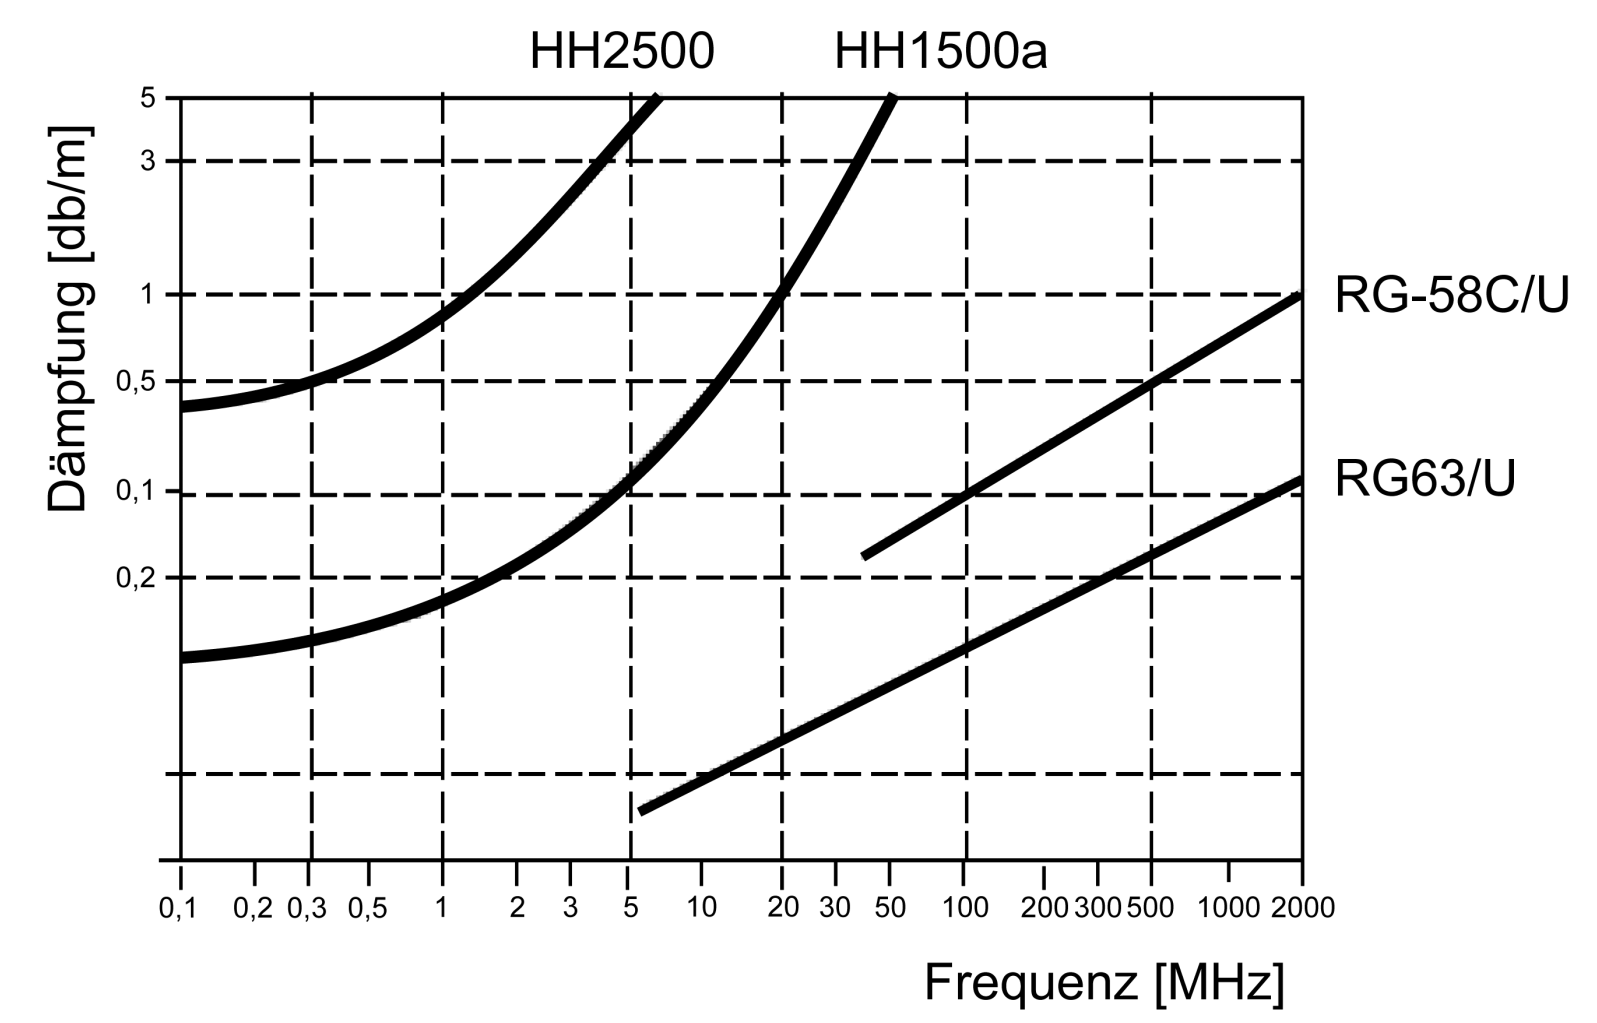
\includegraphics[width=0.7\textwidth]{literatur.png}
        \caption[Literatur Dämpfung pro Meter]{Literaturwerte der Dämpfung pro Meter in Abhängigkeit der Frequenz verschiedener Kabel}\label{fig:literatur}
\end{figure}

\clearpage
\section{Fazit}
In diesem Versuch wurde die Verhaltensweise eines Differenzierglieds untersucht, indem ein Rechtecksignal differenziert worden ist, und die Änderung der Abklingzeit aufgrund verschiedener Widerstände beobachtet wurde.\\\\
Des Weiteren wurden Impulse auf Kabeln behandelt.
Kabel, die verschiedene Enden besitzen, weisen unterschiedliche Eigenschaften auf.
In abgeschlossenen Kabeln, deren Abschlusswiderstand gleich dem Wellenwiderstand des Kabels ist, werden keine Wellen reflektiert;
in offenen Kabeln werden Wellen mit gleicher Phase reflektiert;
und in kurzgeschlossenen Kabeln werden Wellen mit umgekehrter Phase reflektiert.\\\\
Im letzten Versuchsteil wurde sich mit Klippkabeln und der spezifischen Dämpfung beschäftigt.
Wenn ein Rechtecksignal in ein Klippkabel geleitet wird, kann man erkennen, dass es zu sowohl konstruktiver als auch destruktiver Interferenz der beiden Wellen kommt.
Diese sind auch bei verschiedenen Abschlüssen zu erkennen.
Zum Schluss wurde die spezifische Dämpfung des Klippkabels HH2500 auf $D=0.458$ bestimmt und mit dem Literaturwert erfolgreich verglichen. 

\clearpage
\listoffigures
\listoftables
\bibliographystyle{plain}
\bibliography{refs}

%}}}

\end{document}
